\documentclass[a4paper]{article}

\usepackage{../mathstemplate}

\date{IV семестр, весна 2026 г.}
\title{Кластерные алгебры и кластерные категории.\\ Неофициальный конспект}
\author{Лектор: Михаил Александрович Антипов\\ Конспектировал Леонид Данилевич}

\begin{document}
    \shorthandoff{"}
    \maketitle
    \tableofcontents
    \newpage
    \setcounter{lection}{0}
    \newlection{11 февраля 2026 г.}
    \section{Примеры}
    \setcounter{subsection}{-1}
    \subsection{Пентагональная рекуррента}
    Рассмотрим рекурренту $(x_n)_{n \in \N}$ с начальными данными $x_1 = x$, $x_2 = y$, заданную соотношениями $x_{i-1}x_{i+1} = x_i + 1$ (где сами $x_i \in K(x, y)$ для некоторого поля $K$).

    Посчитаем первые несколько членов:
    \begin{align*}x_1 &= x \\ x_2 &= y \\ x_3 &= \frac{y + 1}{x} \\ x_4 &= \frac{x + y + 1}{xy} \\ x_5 &= \frac{x + 1}{y} \\ x_6 &= x \\ x_7 &= y \\ \vdots\end{align*}
    Рекуррента зациклилась за $5$ шагов.

    Можно пытаться рассматривать вариации рекуррентного соотношения вида $x_{i-1}x_{i+1} = x_i^a + 1$, где скажем $a \in \N$.
    Оказывается, она будет циклической только в случаях $a = 1, 2, 3$, и это соответствует тому, что в ранге $2$ есть три системы корней --- $\mathsf{A}_2$, $\mathsf{B}_2 = \mathsf{C}_2$ и $\mathsf{G}_2$.

    Это простейший пример кластерной алгебры: в данном случае имеется кластер из двух переменных, которые по очереди мутируют:
    \[(x_1, x_2) \leftrightsquigarrow (x_3, x_2) \leftrightsquigarrow (x_3, x_4) \leftrightsquigarrow (x_5, x_4) \leftrightarrow \dots\]
    При этом две мутации одной и той же переменной подряд ничего не меняют.

    В общем случае вместо такого пути будет регулярное дерево степени $n$, полное определение мы дадим позже~(\cref{cluster-algebra}).
    \setcounter{subsection}{1}
    \subsection{Фризы Кокстера --- Конвея}
    Фризы Кокстера --- Конвея --- частный случай $\SL_2$-tilings ($\SL_2$-замощения?).
    \definition[$\SL_2$-замощение]{Отображение $f: \Z^2 \to \Q$ с условием $f(i+1,j+1)f(i,j) - f(i,j+1)f(i+1,j) = 1$. }
    \definition[Фриз Кокстера --- Конвея ранга $n$]{
    $\SL_2$-замощение $f$ такое, что \[f(i, j) = \all{0,&i + j < 0 \\ 1,&i + j = 0 \\ 1,&i+j = n+1 \\ 0,&i + j > n+1}\]
    }
    Графически его изображают повёрнутым на $45^o$, вот так:
    \[\cdots\begin{array}{ccccccc}
          \hline
          1 && 1 && 1 && 1\\
          & a^1_1 && a^1_2 && a^1_3 &\\
          a^2_0 && a^2_1 && a^2_2 && a^2_3 \\
          & a^3_0 && a^3_1 && a^3_2 &\\
%          \hline
          &&&\ddots &&& \\
%          \hline
          1 && 1 && 1 && 1 \\
          \hline
    \end{array}\cdots \qquad \begin{array}{c}\begin{array}{ccc}
                                             &b& \\
                                             a&&d\\
                                             & c &
    \end{array}\\\text{должно быть выполнено } ad - bc = 1\end{array}\]
    \example[Фриз ранга $3$]{
    \[
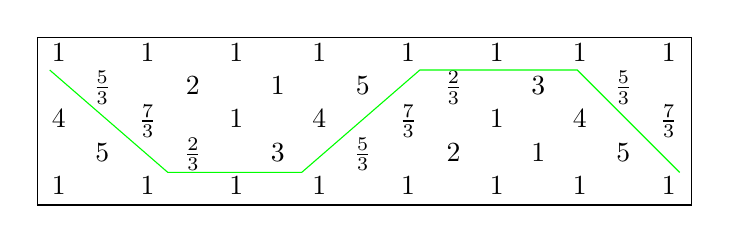
\begin{tikzpicture}
    \node (table){ $\begin{array}{|ccccccccccccccc|}
                        \hline
                        1 && 1 && 1 && 1 && 1 && 1 && 1 && 1\\
                        & \frac53 && 2 && 1 && 5 && \frac23 && 3 && \frac53 &\\
                        4 && \frac73 && 1 && 4 && \frac73 && 1 && 4 && \frac73 \\
                        & 5 && \frac23 && 3 && \frac53 && 2 && 1 && 5 &\\
                        1 && 1 && 1 && 1 && 1 && 1 && 1 && 1\\
                        \hline
    \end{array}$};
    \draw[green] (-4, 0.65) -- (-2.5, -0.65) -- (-0.8, -0.65) -- (0.7, 0.65) -- (2.7, 0.65) -- (4, -0.65);
\end{tikzpicture}
    \]
    Как видно из картинки, фриз имеет ось скользящей симметрии со сдвигом на $\frac{n + 3}{2}$ и переворотом (основания трапеции равны $n + 1$ и $2$).
    Позже это будет видно из классификации в~\ref{freeze-classification}. \comment{Ну, надо что-то ещё потребовать, например, положительности всех элементов фриза хватит.
        А то, кажется, можно при желании составить башню из нескольких фризов произвольного размера, поставленных друг на друга.}
    }
    \exercise[Эффект лорановости]{
    Построим фриз сверху вниз, заполнив верхнюю строчку $a^1_*$ произвольно, и выражая элементы снизу через элементы сверху.
    Тогда если все $a^1_* \in \Z$, то и все элементы снизу тоже (это верно даже в большей общности, тут неважно, что это фриз, то есть что на каком-то уровне снизу будет строка единиц, а потом начнутся нули).
    }
    \theorem[Фриз, построенный по триангуляции]{
    Пусть $T$ --- триангуляция правильного $n$-угольника:
        \[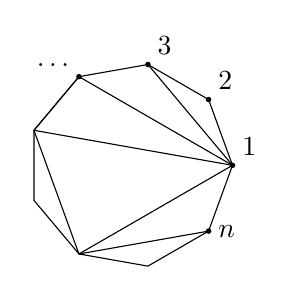
\begin{tikzpicture}
              \pgfmathsetmacro{\R}{1.3};
              \coordinate (A) at ({\R * cos(0)}, {\R * sin(0)});
              \coordinate (B) at ({\R * cos(40)}, {\R * sin(40)});
              \coordinate (C) at ({\R * cos(80)}, {\R * sin(80)});
              \coordinate (D) at ({\R * cos(120)}, {\R * sin(120)});
              \coordinate (E) at ({\R * cos(160)}, {\R * sin(160)});
              \coordinate (F) at ({\R * cos(200)}, {\R * sin(200)});
              \coordinate (G) at ({\R * cos(240)}, {\R * sin(240)});
              \coordinate (H) at ({\R * cos(280)}, {\R * sin(280)});
              \coordinate (I) at ({\R * cos(320)}, {\R * sin(320)});
              \draw plot [smooth cycle, tension=0] coordinates { (A) (B) (C) (D) (E) (F) (G) (H) (I) };
              \draw plot [smooth cycle, tension=0] coordinates { (A) (D) (E) (G) };
              \fill[black] (A) circle (1pt) node[above right]{$1$};
              \fill[black] (B) circle (1pt) node[above right]{$2$};
              \fill[black] (C) circle (1pt) node[above right]{$3$};
              \fill[black] (D) circle (1pt) node[above left]{$\dots$};
              \fill[black] (I) circle (1pt) node[right]{$n$};
              \draw[-] (A) -- (E);
              \draw[-] (A) -- (C);
              \draw[-] (G) -- (I);
        \end{tikzpicture}\]
        Строчка $a^1_i \in \Z$ соответствует фризу (то есть через какая-то строчка снизу будет полностью состоять из единиц) тогда и только тогда, когда $a^1_i$ --- количество треугольников, касающихся вершины $i$ (индексы берутся по модулю $n$).
    Например, триангуляции на рисунке соответствует фриз
    \[\begin{array}{|cccccccccccccccccc|}
    \hline
    1 && 1 && 1 && 1 && 1 && 1 && 1 && 1 && 1 &\\
    & 5 && 1 && 2 && 2 && 3 && 1 && 4 && 1 && 2\\
    9 && 4 && 1 && 3 && 5 && 2 && 3 && 3 && 1 &  \\
    & 7 && 3 && 1 && 7 && 3 && 5 && 2 && 2 && 4\\
    3 && 5 && 2 && 2 && 4 && 7 && 3 && 1 && 7 & \\
    & 2 && 3 && 3 && 1 && 9 && 4 && 1 && 3 && 5 \\
    3 && 1 && 4 && 1 && 2 && 5 && 1 && 2 && 2 & \\
    & 1 && 1 && 1 && 1 && 1 && 1 && 1 && 1 && 1\\
    \hline
\end{array}\]
    \prove[Доказательство в более простую сторону]{
    Рассмотрим двудольный граф $\Gamma$. В левой доле $n$ вершин, соответствующих вершинам многоугольника, а в правой --- $n+1$ вершина, соответствующая треугольнику.
        Проведём ребро, если вершина является вершиной треугольника.

        Пусть $m_{ij}$ --- количество совершенных паросочетаний (из $n + 1$ ребра), где в левой доле взяты все вершины, кроме $i$ и $j$.

    Ясно, что $m_{i,i+1} = 1$: это ребро какого-то треугольника, значит, этот треугольник берётся в паросочетание вместе с оставшейся третьей вершиной; после этого многоугольник разваливается на два, и дальше опять же все по индукции предопределено однозначно:
    \[\begin{tikzpicture}
    \draw plot [smooth cycle, tension=0] coordinates { (A) (B) (C) (D) (E) (F) (G) (H) (I) };
    \draw plot [smooth cycle, tension=0] coordinates { (A) (D) (E) (G) };
    \fill[lightgray] plot [smooth cycle, tension=0] coordinates { (A) (D) (E) };
    \fill[black] (A) circle (1pt);
    \fill[black] (D) circle (1pt) node[above left]{$i$};
    \fill[black] (E) circle (1pt) node[left]{$i+1$};
    \draw[-] (A) -- (E);
    \draw[-] (A) -- (C);
    \draw[-] (G) -- (I);
\end{tikzpicture}\]
    Аналогично проверяется, что $m_{i-1,i+1} = a_i^1$ ($i$-я вершина стоит в паре с любым из инцидентных ей треугольников, после чего остальное предопределено однозначно).

    Осталось применить лемму о конденсации, доказательством которой мы утруждать себя не будем:
    \lemma[О конденсации]{
    Пусть $\Gamma$ --- плоский двудольный граф с левой долей $V_1$ и правой $V_2$, причём $|V_1| = |V_2| + 2$.
    Пусть $i, j \in V_1$. Обозначим через $m_{ij}$ количество совершенных паросочетаний между $V_1 \setminus \{i, j\}$ и $V_2$.
    Если $a, b, c, d \in V_1$ лежат на грани данного графа в этом циклическом порядке (и, разумеется, между ними при обходе грани есть ещё какие-то вершины графа), то выполнено соотношение
        \[m_{ab}m_{cd} + m_{bc}m_{ad} = m_{ac}m_{bd}\qedhere\]
    }
    }
    }
    Соотношение из леммы о конденсации напоминает теорему Птолемея из школьной планиметрии:
    \intfact[Теорема Птолемея]{
        У вписанного четырёхугольника произведение длин диагоналей равно сумме произведений противоположных сторон.
    }
    Также такой вид имеют соотношения в грассманиане.

    \subsection{Координаты на грассманиане и триангуляции}
    Пусть $K$ --- поле.
    Вспомним грассманиан $\Gr(k, n)$ --- многообразие, параметризующее $k$-мерные подпространства в $n$-мерии (например, в пространстве строк $\ind{^n}{K}{}$).

    Грассманиан удобно представлять себе, как множество матриц $M_{k \times n}(K)$ с точностью до действия $\GL_k(K)$ умножениями слева.

    Однородными координатами на грассманиане служат значения миноров $k \times k$, на которые накладываются соотношения Плюккера.
    В случае $k = 2$ эти соотношения выглядят следующим образом:
    \[p_{ik}p_{j\ell} = p_{ij}p_{k\ell} + p_{jk}p_{i \ell}\label{plucker}\tag{$\star$}\]
    где $i < j < k < \ell$, а $p_{ij} = p_{ji}$ равен значению квадратного минора из $i$-го и $j$-го столбца.
    Иными словами, для матрицы $x$: $p_{ij} = x_{1,\min(i, j)}x_{2,\max(i, j)} - x_{1,\max(i, j)}x_{2,\min(i, j)}$.
    Изображая это правило на картинке, получаем правило Птолемея:
    \[\begin{tikzpicture}
          \fill[lightgray] plot [smooth cycle, tension=0] coordinates { (A) (D) (E) (G) };
          \draw plot [smooth cycle, tension=0] coordinates { (A) (D) (E) (G) };
          \draw[-] (A) -- (E);
          \draw[-] (D) -- (G);
          \fill[black] (A) circle (1pt) node[above right]{$i$};
          \fill[black] (D) circle (1pt) node[above right]{$j$};
          \fill[black] (E) circle (1pt) node[left]{$k$};
          \fill[black] (G) circle (1pt) node[below]{$\ell$};
    \end{tikzpicture}\]
    Из картинки ясно, что на самом деле имеет значение только циклический порядок индексов $i, j, k, \ell \in \Z/n\Z$.

    \newlection{18 февраля 2026 г.}
    Размерность многообразия $\Gr(2, n)$ равна $2n - 4$, а размерность Крулля однородного координатного кольца $K[\Gr(2, n)] = K[p_{ij}]/\eqref{plucker}$ на единичку больше, значит, $2n - 3$.
    \definition[Матрица $A \in M_{m\times n}(\R)$ вполне положительна]{Все миноры $A$ положительны.}
    Заинтересуемся схожим вопросом: когда все миноры $2 \times 2$ в матрице $2 \times n$ положительны?
    Более точно, сколько миноров надо проверить на положительность, чтобы положительность остальных последовала?

    Из описания координатного кольца грассманиана ясно, что миноры матрицы --- любые $p_{ij} \in K$, удовлетворяющие соотношениям~\eqref{plucker}.
    Так как $\dim\R[\Gr(2, n)] = 2n - 3$, то такова и степень трансцендентности его поля частных, откуда ответ хотя бы $2n - 3$. \comment{Это видимо не совсем строгое утверждение, так как $\R$ не алгебраически замкнуто.}
    С другой стороны, эта оценка достигается:
    \proposal{\label{plucker-recovery}
    Пусть $T$ --- триангуляция правильного $n$-угольника (множество неупорядоченных пар вершин, соединённых ребром, в том числе пары соседних вершин).
        Пусть $P \coloneqq \defset{p_{ij}}{(i,j)\in T}$
        Тогда любой $p_{rs}$ выражается в виде некоторой рациональной функции от элементов $P$ с положительными коэффициентами.
    В частности, положительность элементов $P$ повлечёт положительность всех миноров $2 \times 2$.
    \prove{Рассмотрим граф, вершины которого --- триангуляции $n$-угольника, а рёбра соответствуют \emph{флипам} следующего вида:
        \[\begin{tikzpicture}[baseline=(current bounding box.center)]
              \fill[lightgray] plot [smooth cycle, tension=0] coordinates { (A) (D) (E) (G) };
              \draw plot [smooth cycle, tension=0] coordinates { (A) (D) (E) (G) };
              \draw plot [smooth cycle, tension=0] coordinates { (A) (B) (C) (D) (E) (F) (G) (H) (I) };
              \fill[black] (A) circle (1pt) node[above right]{$1$};
              \fill[black] (B) circle (1pt) node[above right]{$2$};
              \fill[black] (C) circle (1pt) node[above right]{$3$};
              \fill[black] (D) circle (1pt) node[above left]{$\dots$};
              \fill[black] (I) circle (1pt) node[right]{$n$};
              \draw[-] (A) -- (C);
              \draw[-] (G) -- (I);
              \draw[-] (D) -- (G);
        \end{tikzpicture}\qquad\rightsquigarrow\qquad\begin{tikzpicture}[baseline=(current bounding box.center)]
              \fill[lightgray] plot [smooth cycle, tension=0] coordinates { (A) (D) (E) (G) };
              \draw plot [smooth cycle, tension=0] coordinates { (A) (D) (E) (G) };
              \draw plot [smooth cycle, tension=0] coordinates { (A) (B) (C) (D) (E) (F) (G) (H) (I) };
              \fill[black] (A) circle (1pt) node[above right]{$1$};
              \fill[black] (B) circle (1pt) node[above right]{$2$};
              \fill[black] (C) circle (1pt) node[above right]{$3$};
              \fill[black] (D) circle (1pt) node[above left]{$\dots$};
              \fill[black] (I) circle (1pt) node[right]{$n$};
              \draw[-] (A) -- (C);
              \draw[-] (G) -- (I);
              \draw[-] (A) -- (E);
        \end{tikzpicture}\]
    А именно, любая хорда триангуляции является ребром двух смежных треугольников, в объединении дающих четырёхугольник.
        Назовём \emph{флипом} замену данной хорды триангуляции на другую диагональ четырёхугольника.
        Кстати, этот граф является остовом $(n-3)$-мерного ассоциэдра.

    Ясно, что любая хорда $n$-угольника лежит в какой-то триангуляции.
        Без доказатеельства утверждается, что граф триангуляций связен. Начнём с триангуляции $T$, и, применяя флипы, дойдём до триангуляции, содержащей хорду $r-s$.
        Легко видеть, что $p_{ik}$, где $i-k$ --- хорда, появляющаяся после флипа, выражается через остальные $p_{j\ell}$, отвечающие хордам, присутствовавшим до флипа:
    \[p_{ik} = \frac{p_{ij}p_{k\ell} + p_{jk}p_{i \ell}}{p_{j\ell}}\qquad
    \begin{tikzpicture}[baseline=(current bounding box.center)]
         \fill[lightgray] plot [smooth cycle, tension=0] coordinates { (A) (D) (E) (G) };
         \draw plot [smooth cycle, tension=0] coordinates { (A) (D) (E) (G) };
         \draw[-] (A) -- (E);
         \draw[-] (D) -- (G);
         \fill[black] (A) circle (1pt) node[above right]{$i$};
         \fill[black] (D) circle (1pt) node[above right]{$j$};
         \fill[black] (E) circle (1pt) node[left]{$k$};
         \fill[black] (G) circle (1pt) node[below]{$\ell$};
    \end{tikzpicture}\qedhere\]
    }
    }

    Эту теорему можно пытаться обобщать на разные интересные случаи --- рассматривать не только триангуляции, или скажем работать не на плоскости (или её компактификации --- сфере), а на поверхности с большим числом ручек.
    Впрочем, начиная с некоторого места она уже перестаёт быть верной.

    Ещё пару слов про флипы и триангуляции: можно считать, что диагонали пронумерованы от $1$ до $n - 3$, и при флипе новая диагональ нумеруется тем числом, что было написано на стираемой.
    Тогда получается, что на множестве триангуляций действует свободное произведение $\underbrace{C_2 * \ldots * C_2}_{n}$.

    Действие, разумеется, не свободное.
    Например, флипы диагоналей, далеко друг от друга отстоящих, коммутируют.
    Сами пометки на диагоналях тоже могут перемещаться:
    \exercise{
    Получите последовательностью пяти флипов из одной триангуляции шестиугольника другую:
        \[\begin{tikzpicture}[baseline=(current bounding box.center)]
            \pgfmathsetmacro{\R}{1.3};
            \coordinate (BC) at ({\R * cos(60)}, {\R * sin(60)});
            \coordinate (EF) at ({\R * cos(180)}, {\R * sin(180)});
            \coordinate (HI) at ({\R * cos(300)}, {\R * sin(300)});
            \fill[lightgray] plot [smooth cycle, tension=0] coordinates { (A) (BC) (D) (EF) (G) (HI) };
            \draw plot [smooth cycle, tension=0] coordinates { (A) (BC) (D) (EF) (G) (HI) };
            \draw[-] (A) -- (D) node [midway, above] {$1$};
            \draw[-] (D) -- (G) node [midway, left] {$2$};
            \draw[-] (G) -- (A) node [midway, below] {$3$};
        \end{tikzpicture}\qquad\rightsquigarrow\qquad\begin{tikzpicture}[baseline=(current bounding box.center)]
           \fill[lightgray] plot [smooth cycle, tension=0] coordinates {(A) (BC) (D) (EF) (G) (HI)};
           \draw plot [smooth cycle, tension=0] coordinates {(A) (BC) (D) (EF) (G) (HI) };
           \draw[-] (A) -- (D) node [midway, above] {$1$};
           \draw[-] (D) -- (G) node [midway, left] {$3$};
           \draw[-] (G) -- (A) node [midway, below] {$2$};
        \end{tikzpicture}\]
    }
    \subsection{Классификация фризов}
    \label{freeze-classification}
    Пусть $p \in \Gr(2, n)$ --- точка с однородными координатами $p_{ij}$; предположим, что для всех $i \in \Z/n\Z$: $p_{i,i+1} = 1$.
    Можно составить фриз из координат этой точки следующим образом:
    \[\cdots\begin{array}{ccccccc}
          \hline
          1 && 1 && 1 && 1\\
          & p_{1,3} && p_{2,4} && p_{3,5} &\\
          p_{n,3} && p_{1,4} && p_{2,5} && p_{3,6} \\
          & p_{n,4} && p_{1,5} && p_{2,6} &\\
          &&&\ddots &&& \\
          & p_{?,?-2} && p_{?+1,?-1} && p_{?+2,?} & \\
          1 && 1 && 1 && 1 \\
          \hline
    \end{array}\cdots\]
    $\SL_2$-соотношения выполнены, так как в них превращается соотношение~\eqref{plucker}:
    \[\begin{array}{ccc}
          &p_{i+1,j}& \\
          p_{i,j}&&p_{i+1,j+1}\\
          & p_{i,j+1} &
    \end{array}
    \qquad\begin{tikzpicture}[baseline=(current bounding box.center)]
          \draw[dashed] (-2,-1.5) -- (-2,1.5);
          \draw plot [smooth cycle, tension=0] coordinates { (BC) (D) (EF) (G) };
          \fill (BC) circle (1pt) node[above right]{$i$};
          \fill (D) circle (1pt) node[above right]{$i+1$};
          \fill (D) circle (1pt) node[above right]{$i+1$};
          \fill (EF) circle (1pt) node[left]{$j$};
          \fill (G) circle (1pt) node[left]{$j+1$};
          \draw[dashed] (1.4,-1.5) -- (1.4,1.5);
    \end{tikzpicture}\qquad
    p_{i,j}p_{i+1,j+1} - p_{i+1,j}p_{i,j+1} = p_{i,i+1}p_{j,j+1} = 1
    \]
    Обратно, если есть некоторый фриз, то можно построить числа $p_{ij}$, удовлетворяющие соотношениям Плюккера: пройдём зигзагом вниз по фризу, и положим значения координат, соответствующим зигзаг-триангуляции, равными $q_i$, а остальные восстановим как в~(\cref{plucker-recovery}).
    \[\cdots\begin{array}{ccccccc}
                \hline
                1 && 1 && 1 && 1\\
                & q_1 && \square && \square &\\
                q_2 && \square && \square && \square \\
                & q_3 && \square && \square &\\
                \hline
                &&&\ddots &&& \\
                \hline
                & q_{n-3} && \square && \square & \\
                1 && 1 && 1 && 1 \\
                \hline
    \end{array}\cdots\qquad\begin{tikzpicture}[baseline=(current bounding box.center)]
           \draw plot [smooth cycle, tension=0] coordinates { (A) (B) (C) (D) (E) (F) (G) (H) (I) };
           \draw[-] (D) -- (B) -- (E) -- (A) -- (F) -- (I) -- (G);
    \end{tikzpicture}\]
    Далее остальные значения во фризе восстанавливаются однозначно из $\SL_2$-соотношений, и в силу выше построенного примера, они все будут иметь вид $p_{ij}$.
    Единственность на самом деле имеет место чуть более слабая --- например, она есть если все $q_i > 0$ --- тогда~\cref{plucker-recovery} говорит, что все полученные координаты будут положительными.
    Значит, на самом деле фриз однозначно восстанавливается по $q_i$ и на некотором открытом по Зарисскому множестве.
    \note{
    Отсюда получается, что при условии $p_{i,i+1} = 1$ для всех $i \in \Z/n\Z$ точка лежит на грассманиане, если выполнены уравнения
    \[p_{i,j}p_{i+1,j+1} - p_{i+1,j}p_{i,j+1} = 1.\]
        \comment{По-видимому, если ещё подумать, отсюда следует, что вместо всех соотношений грассманиана достаточно проверять соотношения
        \[p_{i,j}p_{i+1,j+1} - p_{i+1,j}p_{i,j+1} = p_{i,i+1}p_{j,j+1},\]
        но я не уверен}.
    }
    \section{Определения}
    \subsection{Колчаны и кластерные матрицы}
    \definition[Колчан]{Произвольный ориентированный граф $Q = (V, E)$, в котором всё разрешено: петли, кратные рёбра, может быть даже бесконечное число вершин или рёбер\ldots}
    \definition[Кластерный колчан]{Конечный колчан без петель и рёбер туда-обратно (пары рёбер вида $i \to j$ и $j \to i$).}

    Кластерные колчаны $Q$ взаимно однозначно соответствуют кососимметрическим матрицам: колчану $Q$ отвечает матрица $B_Q \in M_{n}(\Z)$ (где $n = |V|$):
    \[(B_Q)_{i,j} = \all{\#\{i \to j\},& \text{ есть стрелки $i \to j$} \\ \#\{j \to i\},& \text{ есть стрелки $j \to i$}\\0,&\text{иначе}}\]
    \definition[Кластерный колчан с замороженными вершинами]{
        Кластерный колчан на $m$ вершинах, где первые $n \le m$ вершин называются \emph{незамороженными}, а последние $m - n$ вершин называются \emph{замороженными}, и между ними нет рёбер.
    }
    На матричном языке кластерный колчан с замороженными вершинами изображают в виде матрицы $\tilde{B} \in M_{m\times n}(\Z)$, где $\tilde{B} = \vect{B\\\hline C}$, и $B \in M_{n}(\Z)$ кососимметрическая, а $C \in M_{(m-n) \times n}(\Z)$ --- любая.
    Теоретически можно было бы считать, что кластерному колчану с замороженными вершинами отвечает кососимметрическая матрица из $M_{m}(\Z)$, где правый нижний квадрат $(m - n) \times (m - n)$ нулевой, но так уже не поступить с обобщением данного понятия --- \emph{кластерными матрицами}, которые мы определим чуть позже.


    Пусть $Q$ --- конечный кластерный колчан, $1 \le i \le n$ --- незамороженная вершина.
    \definition[Мутация $Q$ в вершине i]{
        На колчанном языке это новый колчан $M_i(Q)$, в котором множество вершин то же самое, а множество рёбер претерпевает следующие изменения:
    \numbers{
        \item Для каждой пары вершин $k, \ell$, таких, что есть рёбра $k \to i \to \ell$, добавляем ребро $k \to \ell$ (если рёбер $k \to i$ всего $n_k$ штук, а рёбер $i \to \ell$ всего $n_\ell$ штук, то мы добавим $n_k \cdot n_\ell$ рёбер.
        \item Разворачиваем стрелки, инцидентные $i$.
        \item Стираем всевозможные противонаправленные пары (если было $n$ рёбер в одну сторону, и $m$ в другую, то останется $\abs{n - m}$ понятно в какую сторону).
    }
    }
    На матричном языке мутация выглядит так: из $B_Q = (b_{ij})$ получается $B_{M_i(Q)} \eqqcolon M_i(B_Q) = (b'_{ij})$:
    \[b'_{pq} = \all{-b_{pq}, & i = p \text{ или } i = q \\ b_{pq} + b_{pi}b_{iq},& b_{pi}, b_{iq} > 0 \\ b_{pq} - b_{pi}b_{iq} ,& b_{pi}, b_{iq} < 0 \\ b_{pq} ,&\text{иначе}}\tag{$\triangle$}\label{mutation}\]

    \note{Это инволюция: две мутации подряд в одной и той же вершине не меняют колчан.}
    \example{Пусть $v$ --- сток или исток. Мутация в вершине $v$ --- разворот рёбер, инцидентных $v$.}
%    // времени много прошло сегодня... Ладно, может хотя бы определение кластерной алгебры дадим сегодня. (18:14)
    \exercise{Если $Q$ --- дерево на $n$ вершинах, то мутациями в истоках и стоках можно получить любую ориентацию всех $n - 1$ рёбер.}
    Этот факт известен даже среди алгебраистов, и отвечает следующему утверждению: категории модулей над некоторыми конечномерными алгебрами почти эквивалентны в некотором смысле, \comment{вроде так}.

    Однако если делать мутации не в источниках и стоках, то даже какой-нибудь путь может претерпевать очень значительные изменения.
    Тем не менее, верен следующий факт:
    \intfact{Пусть $Q_1$ и $Q_2$ --- два кластерных колчана без ориентированных циклов на одном множестве вершин.
    Предположим, что они эквивалентны: существует последовательность мутаций, превращающих один в другой.
    Тогда $Q_2$ получается из $Q_1$ только при помощи мутаций в источниках и стоках. В частности, они изоморфны как неориентированные графы.}
    Что любопытно, комбинаторное доказательство этой теоремы неизвестно, а вот с помощью кластерных категорий доказательство существует уже давно.

    \definition[Матрица $B' \in M_{n}(\mathbb{Z})$ кососимметризуема]{Существуют $D = \mathrm{diag}(d_1, \ldots, d_n)$ при $d_i > 0$ и кососимметричная $B \in M_n(\mathbb{Z})$: $B' D = D B$. }
    Говоря русским языком, кососимметричная матрица с точностю до перемасштабирования строк \comment{Что? Вроде же с точностью до сопряжения\ldots}
    \definition[Кластерная матрица]{$\tilde{B} \in M_{m,n}(\mathbb{Z})$, такая что верхний квадрат $n \times n$ --- кососимметризуемая матрица, а нижний прямоугольник --- любая.}
    Мутацию в незамороженной вершине $1 \le i \le n$ кластерной матрицы определим по формуле\eqref{mutation}.
    \statement{Мутация по-прежнему инволюция; кососимметризуемость верхнего квадрата сохраняется после мутации; $M_i$ коммутирует с транспониованием $B \mapsto B^t$ и разворотом всех рёбер $B \mapsto -B$. Если $b_{ij} = b_{ji}=0$, то мутации $M_i$ и $M_j$ коммутируют при действии на даyную кластерную матрицу.
    \prove{
        Не совсем очевидно, но проверяется в лоб.
    }
    }
    \subsection{Кластерная алгебра}
    \label{cluster-algebra}
    Обозначим через $T_n$ регулярное дерево степени $n$ с неориентированными рёбрами, покрашенными числами $1, \ldots, n$.
    Иными словами, граф Кэли для $\underbrace{C_2 * \ldots * C_2}_{n}$.
    Отметим некоторую вершину $t_0$.

    Теперь пусть $K$ --- поле, $\tilde{B} \in M_{m\times n}(\mathbb{Z})$ --- кластерная матрица.
    Для определения кластерной алгебры нам потребуется следующий набор данных:
    \bullets{
    \item Отображение, сопоставляющее каждой вершине $T_n$ по кластерной матрице $m\times n$, такое что для любых вершин $t_1$ и $t_2$, соединённых ребром цвета $i$, выполнено соотношение $B(t_2) = M_i(B(t_1))$.
        Ясно, что задать такое отображение --- всё равно, что задать кластетрную матрицу для $t_0$, остальные определяются однозначно.
    \item Отображение $x: V(T_n) \to K(x_1, \ldots, x_{m})^m$. Вектор $x(t) = \vect{x_1^t, \ldots, x_m^t}$ называется \emph{расширенным кластером} в вершине $t$, а совокупность всех элементов всех векторов зовётся \emph{кластерными переменными}.
        Первые $n$ переменных расширенного кластера формируют обычный \emph{кластер}.
        При этом $x(t_0) = (x_1, \ldots, x_m)$, и опять же имеется связь между значениями в соседних вершинах: если вершины $t$ и $t'$ соединены ребром цвета $i$, $x(t) = y, x(t') = y'$, и в вершине $i$ стоит матрица $B(t) = (b_{ij})$ то при $j \ne i$: $y_j = y_j'$, а при $j = i$ выполнено соотношение: \[y_i y_i' = \prod_{b_{ki}>0}y_j^{b_{ki}} + \prod_{b_{ki}<0}y_j^{-b_{ki}}.\]
    }
    \definition[Кластерная алгебра $A(B)$]{Подалгебра в $K(x_1, \ldots, x_m)$, порождённая кластерным переменными.}
    И это ещё не самое общее определение, здесь мы определили так называемую \emph{кластерную алгебру геометрического типа}.
    Но других у нас, вероятно, не будет.

    Этот тип называется геометрическим, так как однородное кольцо грассманиана и некоторых других интересных многообразий --- такие кластерные алгебры.
\end{document}
